
\documentclass[sigconf]{acmart}

\usepackage{todonotes}
\usepackage{hyperref}

\usepackage{endfloat}
\renewcommand{\efloatseparator}{\mbox{}} % no new page between figures

\usepackage{booktabs} % For formal tables

\settopmatter{printacmref=false} % Removes citation information below abstract
\renewcommand\footnotetextcopyrightpermission[1]{} % removes footnote with conference information in first column
\pagestyle{plain} % removes running headers

\begin{document}
\title{Mapping Police Killing of Citizens in the United States}

\author{Jeramy Townsley}
\orcid{1234-5678-9012}
\affiliation{%
  \institution{IUPUI}
  \streetaddress{425 University Ave}
  \city{Indianapolis} 
  \state{Indiana} 
  \postcode{46202}
}
\email{jtownsle@indiana.edu}


\begin{abstract}
With the rise of camera phones that allows citizens to videotape law enforcement brutality against citizens, and the ability to immediately make those videos public through social media, there has been an increased awareness of police killings of citizens.  With this new data there have been a number of systematic attempts to document these events, from journalists, to academics, to activists, since there is no credible government database documenting this problem. These events can be mapped at the county level with the open source software QGIS.  Further, demographic and economic data gathered by the Census at the county level can be collected and tested against the police-killings to determine if a regression model can be used to describe a pattern among these variables. 
\end{abstract}

\keywords{i523, hid347, police violence, negative binomial regression, gis mapping, American Community Survey}

\maketitle

\section{Introduction}



\section{Tracking Deaths Caused by Law Enforcement}
There is no central database in the United States for any killings, whether caused by citizens or law enforcement.  The best publicly available government resource is the FBI database on homicides from the Uniform Crime Report (UCR).  However, as numerous sources have documented, this database is unreliable because participation by local and state law enforcement agencies is voluntary. \cite{currie16,pridemore05,dalton17} There have been several attempts by researchers and law enforcement to get a better picture of homicide rates.  For example, the FBI's Supplementary Homicide Report, and National Vital Statistics Systems are two federal-level attempts to collect more detailed statistics, but those efforts are not presumed to represent the entire population of homicides. \cite{pridemore05} What they show is the failure of the UCR to capture all of the relevant data.

Similarly, data on homicides specifically reported to have been committed by law enforcement face similar deficits.  \cite{currie16,pridemore05}  To overcome this problem, journalists, academics, and activist organizations have used publicly available sources to find instances of law enforcement-caused deaths.  For example, the British news agency, {\em The Guardian}, created a two-year project, The Counted, where they manually searched news reports for cases of deaths caused by law enforcement.  \cite{counted}  Additionally, they posted contact information for the public to send them tips about cases not already in their database.  While The Guardian database for 2015-2016 remains available to the public, they discontinued the project, so no 2017 data is available.  It has some interactive features, where the user can filter the data by state where the killing occurred, how the death occurred, whether the victim was alleged to have been armed, victim's gender, race, and age.  Where possible, a picture of the victim and a brief biography is available.  They report that 1,093 people were killed by law enforcement in 2016 alone.

Another new agency that relies on a similar process to capture data about deaths caused by police, is the {\em Washington Post}.  They host an ongoing project that lists only people shot to death by police, Fatal Force, and contains links to the original news stories where the deaths were reported. \cite{fatalforce}  Its numbers are lower than The Counted, which includes any deaths caused by law enforcement, not just shootings.  However, it also notes that its database has more than twice the number of shootings by law enforcement per year than the FBI database.  Like {\em The Guardian}, it has contact information to send new information about killings, as well as photos or videos about the victims.  Their list of victims starts from January 1, 2015.  They report that 963 people were shot to death by law enforcement in 2016.

Mapping Police Violence (MPV) was created by three community activists and organizers.  Their reported methodology is to have used three online databases, and to have compiled those lists into MPV.  Neither {\em The Guardian} or the {\em Washington Post} are reported as a source for MPV for the two years of data available from those agencies. They operationalize police killings as, ` case where a person dies as a result of being chased, beaten, arrested, restrained, shot, pepper sprayed, tasered, or otherwise harmed by police officers, whether on-duty or off-duty, intentional or accidental.' \cite{policeviolence} Their list of victims begins from January 1, 2013.  They report that 1155 people were killed by law enforcement in 2016.  This is the database used for this project to identify the counties where people were killed by law enforcement.

\section{Data and Measures}

All of the variables used in this study can be found in Table 1, as well as a brief definition of each, and basic variable descriptions such as mean and standard deviation.  The dependent variable is a count of the number of people killed in any given county in the United States from January 2013 to October 2017 and was downloaded from the web site, Mapping Police Violence (mappingpoliceviolence.org) on November 5, 2017.  Compared to the two news agencies that have been tracking deaths from law enforcement, their list of victims is more comprehensive for 2016 (1155 vs 963 and 1093), and it covers a longer time-frame, since the news agencies only have data since 2015.  The original downloadable xlsx (Excel) file contained 24 variables on the primary sheet, such as the victim's name, whether the victim was armed, a link to the original news story, whether there were reports of mental illness, the county, zip-code, state, specific address of the killing, victim's age, race, gender, date of the incident, and police department involved in the killing. At the time of download, the spreadsheet contained a total of 5,634 observations, that each represent a killing by law enforcement in the US in approximately the last five years.

\begin{figure}
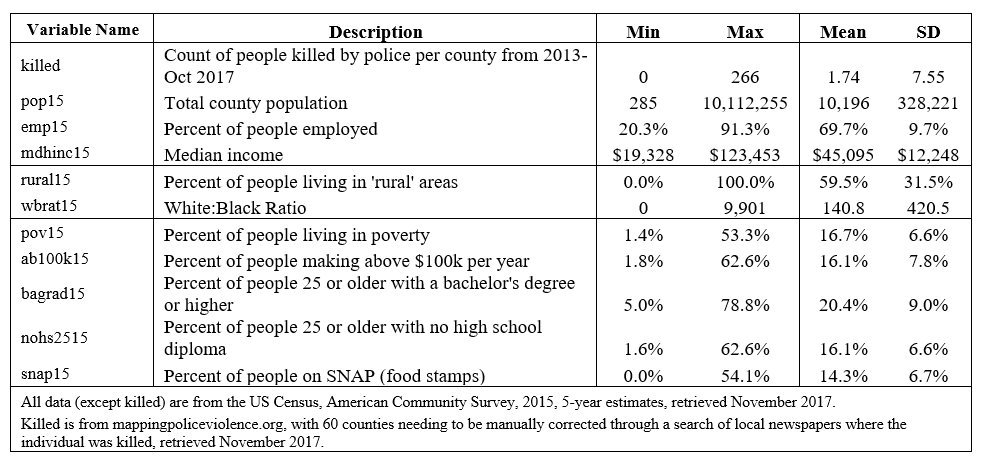
\includegraphics[width=1.0\textwidth]{images/table1.jpg}
\caption{All variables used in this study.}
\end{figure}

This data contained errors that had to be manually corrected.  The errors were discovered when the "killed" variable, count of the number of people killed by law enforcement in any given county, was merged with the Census data that were the independent variables.  The Census data contains an official list of states and counties in those states. The MPV data listed counties that were not in the claimed states.  It was discovered that some were simply errors, some were city coded as county, and some were blank.  Sixty observations total were found to have errors.  Using the victim's name provided by MPV, they were searched using Google in November, 2017, to find an original news story reporting this killing.  Once the killing could be verified, similar investigation confirmed the county and state of the killing.  The corrected data was used for this analysis.  It is possible that other errors exist, since the only errors detected were those where there was no correct match with an actual Census-listed county and state.  There may be counties where a victim is claimed to have been killed, where the county and state exist, but misidentified.  The data has approximately the same number of observations as the two news agencies' data, strengthening its claims to validity.  Further, each of the 60 misspecified counties tracked back to an actual killing by law enforcement based on a search of the victim's name.

The independent variables were all obtained from the United States Census, which maintains a large, publicly-available database on their website. \cite{census}  All of the data used for this study are at the administrative unit of the county, and includes all of the 3142 United States counties listed by the Census.  All of the ten variables were downloaded (November, 2017) from the American Community Survey (ACS). The ACS is a subsidiary of the Census Bureau which administers an extensive survey of an annual sampling of the US population on various economic and demographic questions.  Each of the variables chosen for this project falls into one of five categories: population total, race, education, geography-type and economic.  The total population of each county is estimated by the ACS based on annual census data, and represents a single-year value.  The rest of the variables are estimated from aggregates of data collected from 2011-2015, a five-year estimate.  

The only race variable in this study is a ratio of White:Black population per county.  The Census uses self-identification of the individuals to label race.  Individuals can self-identify as multiple race and ethnic groups.  In this case, only those individuals listing a single race, White or Black, were counted, and a ratio was calculated.  The geography-type variable represents whether a person lives in a rural or urban area.  The census defines {\em urban} as any place with at least 2,500 people, and {\em rural} as everyplace else.  This variable is a percent of the county population who does not live in an urban area.  The two education variables only count those residents who are over 25 years of age, either who have a bachelor's degree or higher, or who do not have a  high-school diploma.  

There are five economic-related variables.  The first, percent of people employed compared to the county population, is taken only from those 20-64 years old.  The second measures the median income per county.  Income can be measured in several different ways, and while mean is a common measure of central tendency, it is often skewed up by high incomes, since low incomes are limited to zero.  Because of this, median income is typically used.  Two variables measure income deficits--the percent of people who have qualified for SNAP (food stamps), and the percent of people living below poverty.  The latter relies on the definition of poverty provided by the Office of Management and Budget, which varies this designation based on size and composition of the family.  The fifth measure is the percent of the population living above \$100,000  per year. The Census lists the median U.S. income at almost \$60,000 per year, and provides the \$100k data as a measure of a high-income county.

In addition to demographic and economic data, the Census Bureau provides a significant amount of geospatial information.  Through their TIGER products (Topologically Integrated Geographic Encoding and Referencing), they provide a web site where the public can download shapefiles at many different levels that are published each year, and can be connected to the rest of their data. \cite{tiger} For this study, county-level data was used, since it was the smallest administrative unit for which all of the data was available.  While accurate state-level data was available, it did not seem fine-grained enough to provide a sufficient analysis.  Smaller administrative levels, like census-tract, and even block-level shapefiles are available, and there is annual census data that can be mapped onto those levels.  While  some ACS variables are available at these small units, they typically only cover a random selection, and can have high error rates.  County-level data is the smallest administrative unit for which every county in the U.S. can be measured in the five-year estimates file.  These shapefile used for this study was the 2015 county-level data for the entire United States.  However, not all places available on the shapefile have data through the ACS.  For example, several of the smaller island territories are not included in the ACS survey, so those are excluded in the map, as well as the regression analysis.  While the latter includes Alaska and Hawaii, for ease of viewing the county-level data, those states are not included on the map (Figure 1).


\section{Methods}



\begin{figure}
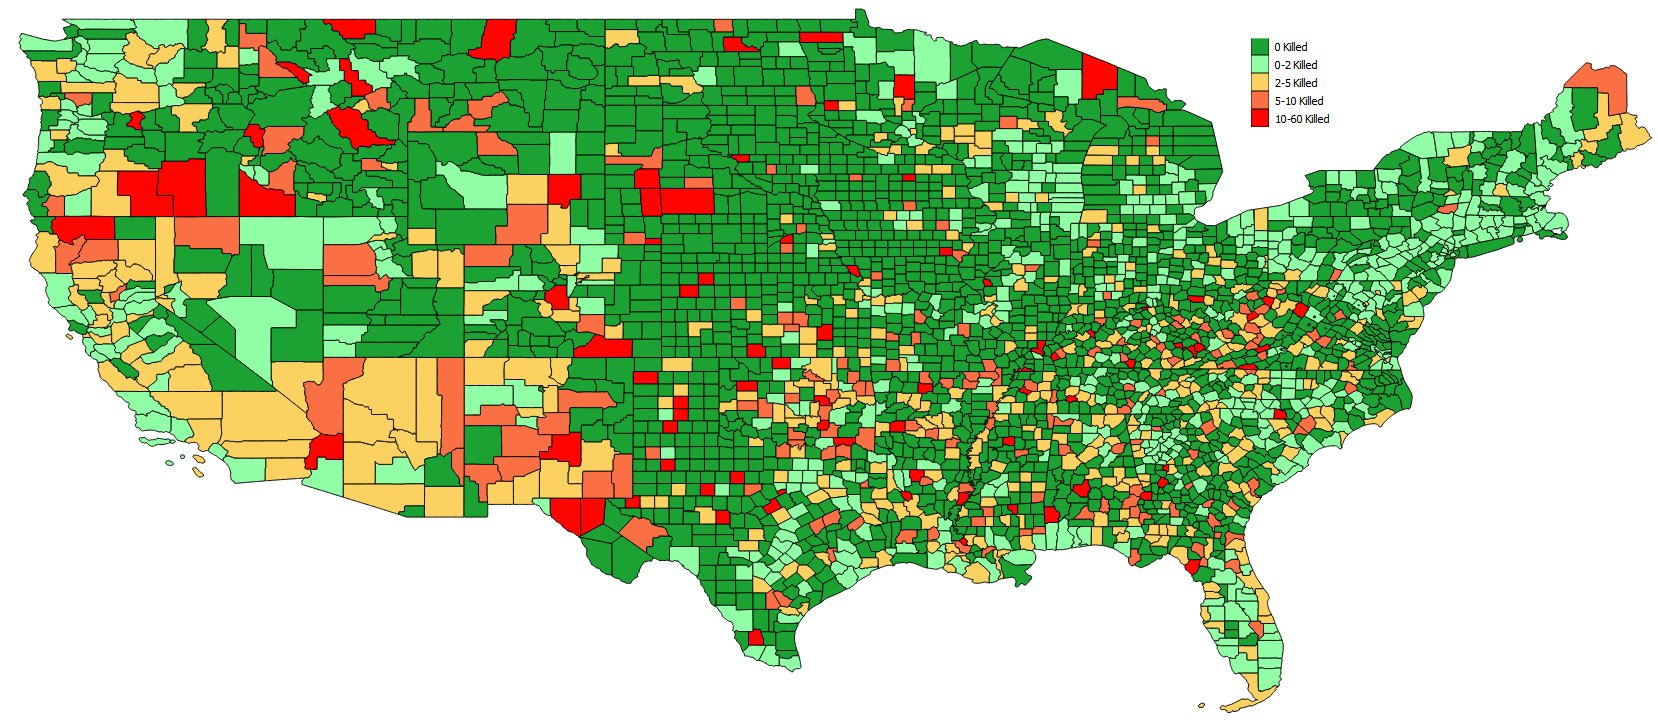
\includegraphics[width=1.0\textwidth]{images/figure1.jpg}
\caption{U.S. county-level map of residents killed by police, 2013-Oct 2017.  Data from Census and mappingpoliceviolence.org}
\end{figure}



\begin{figure}
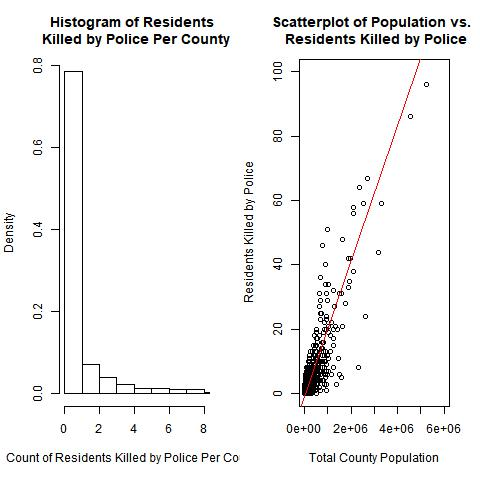
\includegraphics[width=1.0\textwidth]{images/figure4.jpg}
\caption{Left: Histogram of the number of county residents killed by police.  This histogram shows a maximum of eight per county killed by police, while the actual maximum is 266.  However, there are only 120 observations where this value is above 8.  This view gives a better depiction of the data.  Right: Scatter plot of the total county population versus the total killed by police in that county.  The red line is a regression prediction line for these two variables.}
\end{figure}

\begin{figure}
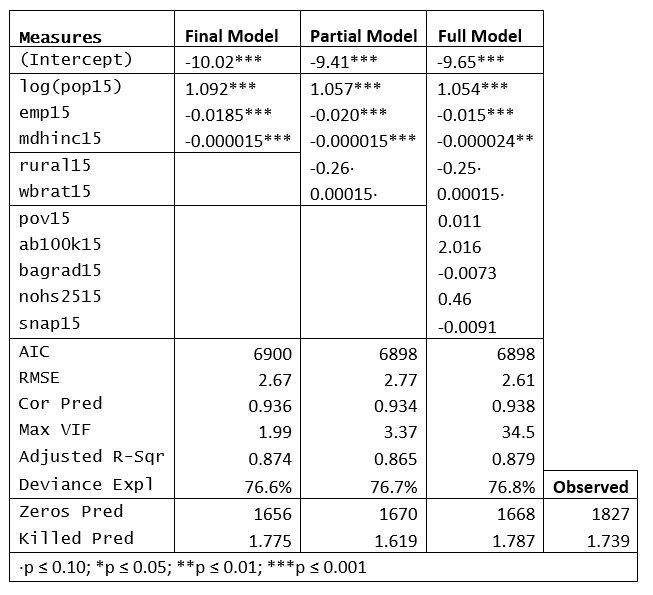
\includegraphics[width=1.0\textwidth]{images/table2.jpg}
\caption{Regression and diagnostic results from all three models.  "Zeros Pred" are the number of counties where no person is predicted to be killed by police, calculated not at exact zero, but any value less than 0.5.  "Killed Pred" is the mean number of predicted people killed by police in each county.}
\end{figure}

\begin{figure}
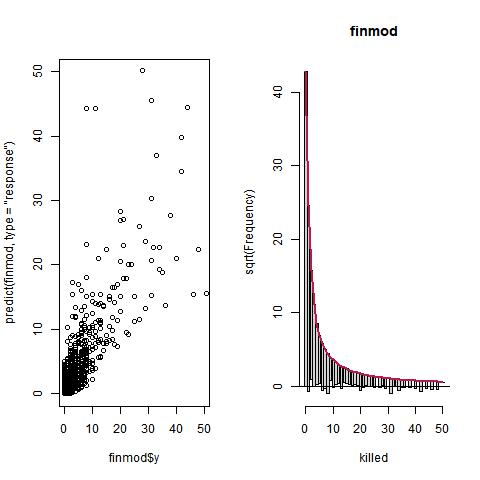
\includegraphics[width=1.0\textwidth]{images/figure2.jpg}
\caption{Left: Scatter plot of predicted versus observed counts of residents killed by police per county. Right: Rootogram--fit of the final regression model: negative binomial with three independent variables (log of population, employment and median income).  The red line can be interpreted as the observed values.  Bars that are hanging below the zero-line are under-fit for that bin, and those above the line are over-fit for that bin.}
\end{figure}

\begin{figure}
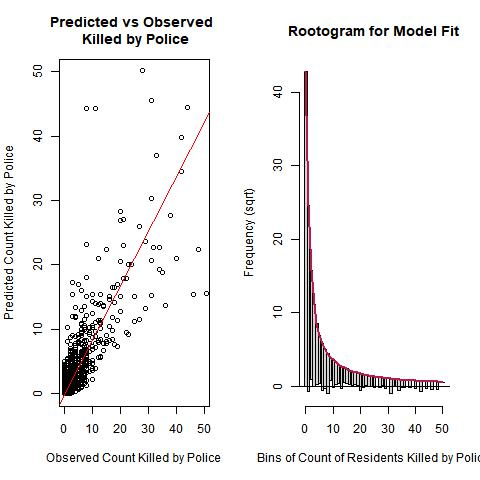
\includegraphics[width=1.0\textwidth]{images/figure3.jpg}
\caption{Regression diagnostics plots for the final model with three independent variables: population (log), employment and median income. Top: Residuals versus fitted and residuals versus index.  Bottom: Quantile residuals and QQ Plot of residuals. }
\end{figure}


\section{Conclusion}
\bibliographystyle{ACM-Reference-Format}
\bibliography{report} 

\end{document}
